%プログラミング応用/ソフトウェア工学 要求仕様書 要求仕様書
\documentclass[11ptm]{jsarticle}

\usepackage{etoolbox}

\usepackage{array}

\usepackage{enumitem}

\usepackage{amsmath, newtxmath}

\usepackage[dvipdfmx]{graphicx}
%\usepackage[draft, dvipdfmx]{graphicx}

\usepackage[hang, small, bf]{caption}
\usepackage[subrefformat=parens]{subcaption}
\captionsetup{compatibility=false}

\usepackage{listings, jlisting}

\lstset{
  basicstyle={\ttfamily\small},
  frame=tbrl,
  breaklines=true,
%  language=C,
  lineskip=-0.5ex,
  tabsize=2
}


\usepackage{tabularx}


\makeatletter
\AtBeginDocument{
\let\c@figure\c@lstlisting
\let\thefigure\thelstlisting
\let\ftype@lstlisting\ftype@figure
}
\makeatother

\title{{\Huge 要求仕様書}\\第4版}
\author{24 高橋祥吾\\26 田桑大輔\\29 田中稀尋\\30 谷川僚}
\date{}

%%%%%%%%%%%%%%%%%%%
%%%%%%%%%%%%%%%%%%%
\begin{document}

\setcounter{page}{0}

\maketitle
\thispagestyle{empty}

\clearpage

\setcounter{page}{0}
\thispagestyle{empty}

\tableofcontents
\clearpage


%%%%%%%%%%%%
\section{ソフトウェアの概要}
\label{sec:ソフトウェアの概要}
本節では, 資産管理システム(仮称)の概要を述べる.

%%%%%%
\subsection{はじめに}
\label{subsec:はじめに}
本ソフトウェアはサレジオ高専で備品を扱う際に使用するソフトウェアである. \par
サレジオ高専での備品の管理は10,000円以上のものを対象に行われており, 対象の備品にID, 種類, 名前, 管理者が書かれたシールを貼り管理している. 現状では備品を管理する際にリストへの追加や削除が簡単に行えないのに加え, 備品が移動した際に再度の登録を行っていないため, 備品の紛失などが起こってしまっている.\par
これを防ぐために, PCやスマートフォンなどの各種端末から容易にアクセス可能で, 備品の情報を簡単に閲覧・更新できるようなソフトウェアを作成する.

%%%%%%
\subsection{作成するソフトウェアの全体像}
\label{subsec:作成するソフトウェアの全体像}
\ref{subsec:はじめに}節で挙げた問題点を技術的に解決できるようなソフトウェアを作成するために, 以下の項目の実装が必要だと考えている.
\begin{enumerate}
  \item 備品データを視覚的に管理・検索・追加・削除・変更を行えるようなプラットフォーム
  \item 備品データを効率的に管理するデータベース
  \item 簡潔明瞭なインターフェース
  \item ユーザ機能(管理者ユーザ, 一般ユーザ)
  \item QRコードなどを活用した, カメラ付き端末からのアクセス
\end{enumerate}


%%%%%%%%%%
\newpage
\section{開発及び動作プラットフォーム}
\label{sec:開発及び動作プラットフォーム}
本ソフトウェアの開発及び動作をするプラットフォームを以下に示す.

%%%%%
\subsection{ソフトウェアの開発環境}
\label{subsec:ソフトウェアの開発環境}
\begin{description}[labelwidth=9em]
  \item[使用言語] HTML, CSS, JavaScript, PHP, MySQL
  \item[使用フレームワーク] XAMPP
  \item[使用ミドルウェア] Git
  \item[使用開発環境] Visual Studio Code, Xcode
\end{description}

\subsection{ソフトウェアの動作プラットフォーム}
\label{subsec:ソフトウェアの動作プラットフォーム}
本ソフトウェアは, インターネットに接続可能で, ブラウザがインストールされている各種端末上で動作する. \par
スタンドアロン(オフライン)でも動作するようにするか, オンライン上での動作に限定するかは未定である.
%\begin{itemize}
%\item ブラウザがインストールされている各種端末
%\end{itemize}


%%%%%%%%%%
\newpage
\section{ソフトウェア全体の構成}
\label{sec:ソフトウェア全体の構成}
本ソフトウェアは, サーバ・クライアント方式のWebアプリケーションでの実装を想定している. そのため, ユーザが操作するWebページとサーバ上のデータベースが存在し, 互いに連携する. \par
\ref{subsec:ソフトウェアの開発環境}節より, それぞれのサイドでは次の言語および開発環境を使用する予定である.
\begin{description}[labelwidth=15em]
  \item[クライアントサイド(Webページ)] HTML, CSS, JavaScript
  \item[サーバサイド] PHP, MySQL
\end{description}
また本ソフトウェアは, \ref{subsec:作成するソフトウェアの全体像}節で挙げた項目において対応する機能およびシステムによって構成される. 対応表を以下に示す.
\begin{table}[h]
  \caption{必要項目に対応する機能}
  \label{tb:必要項目に対応する機能}
  \centering
  \begin{tabularx}{\linewidth}{l|l}
    1.\ 備品データを視... & 登録機能, 削除機能, 変更機能, 検索機能 \\
    \hline
    2.\ 備品データを効... & サーバによるデータベース             \\
    \hline
    3.\ 簡潔明瞭なイン... & Webページ                              \\
    \hline
    4.\ ユーザ機能      & ユーザ登録・ログイン機能             \\
    \hline
    5.\ QRコードなどを... & 未定                                   \\
  \end{tabularx}
\end{table}


%%%%%%%%%%
\newpage
\section{各機能・システムの詳細}
\label{sec:各機能の詳細・システムの詳細}
各機能および各システムについての詳細を以下にまとめる.

%%%%%
\subsection{データの形式}
\label{subsec:データの形式}
本ソフトウェアは資産情報をデジタルデータで扱っていく. この際に必要になる情報の保存形式を次の表\ref{tb:データの形式}に示す.
\begin{table}[h]
  \caption{データの形式}
  \label{tb:データの形式}
  \centering
  \begin{tabular}{@{}l|l|l|l|l@{}}
    項目     & 概要                               & 要求する入力形式 & 登録の可不可     & 変更の可不可 \\
    \hline\hline
    資産番号 & 資産ごとの固有のID                 & システムで生成   & admin       & admin   \\
    \hline
    資産名   & 登録する際の名称. 型番など.        & 文字列     & possible               & admin        \\
    \hline
    形式     & 資産の分類. PCやプリンターなど     & 選択形式または文字列     & possible & admin        \\
    \hline
    所属     & 資産が利用, 所在する所属. 学科など & 選択形式     & possible             & admin        \\
    \hline
    場所     & 資産の所在. 部屋番号を想定         & 選択形式     & possible             & possible     \\
    \hline
    担当     & 資産の所有者および使用者           & 文字列     & possible               & possible     \\
    \hline
    管理者   & 資産の管理者または責任者           & 選択形式または文字列     & possible & admin        \\
    \hline
    個数     & 資産の個数                         & 整数値     & possible               & possible        \\
    \hline
    画像     & 資産の写真またはイメージ図         & 画像のアップロード     & possible   & admin        \\
    \hline\hline
    取得日時 & 資産情報を登録した日時             & システムで生成   & impossible       & impossible   \\
    \hline
    編集日時 & 資産情報に変更を加えた最新の日時   & システムで生成   & impossible       & impossible
  \end{tabular}
\end{table}\par
変更の可不可について, 変更可能性が低いが修正する可能性があるものを, 管理者権限によってのみ変更可能であるとして, adminと表記した.

%%%%%
\subsubsection{補足説明}
\label{subsubsec:補足説明}
資産番号については, 事務だけでなく学科長に申請することで資産購入・登録できるように, 事務および学科長を想定したadmin(管理者ユーザ)が登録および変更できるものとした. \par
個数については, 変更時に任意の量だけ場所の変更などが可能で, 場所が異なる資産については別のデータとして管理されるようになる. 

%%%%%
\clearpage
\subsection{状態遷移図}
\label{subsec:状態遷移図}
本ソフトウェアを実行した際の状態遷移図を次に示す. 図\ref{fig:一般ユーザの状態遷移図}を一般ユーザの状態遷移図, 図\ref{fig:adminの状態遷移図}を管理者ユーザの状態遷移図とする. \par
緑(濃い)色の四角は画面を表しており, 楕円はボタン, 黄(薄い)色は機能を示している.
\begin{figure}[h]
  \centering
  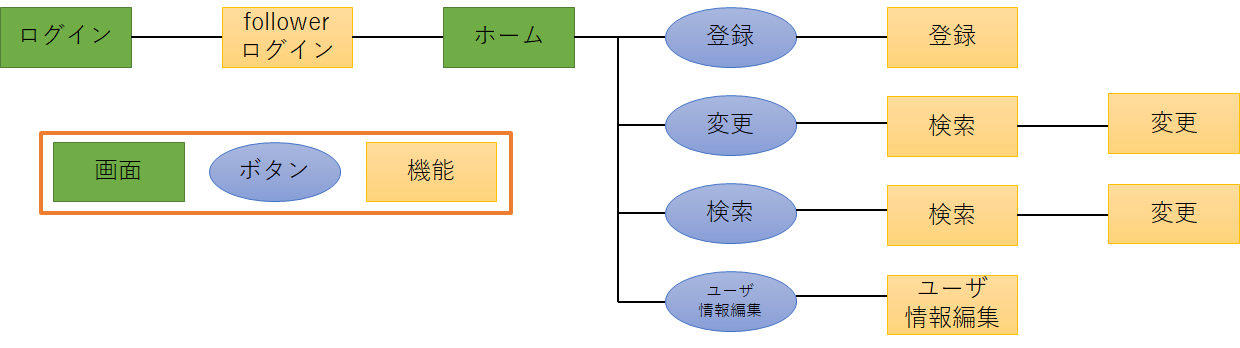
\includegraphics[keepaspectratio, width=0.8\linewidth]{follower_transition-diagram.png}
  \caption{\label{fig:一般ユーザの状態遷移図}一般ユーザの状態遷移図}
\end{figure}\par

\begin{figure}[h]
  \centering
  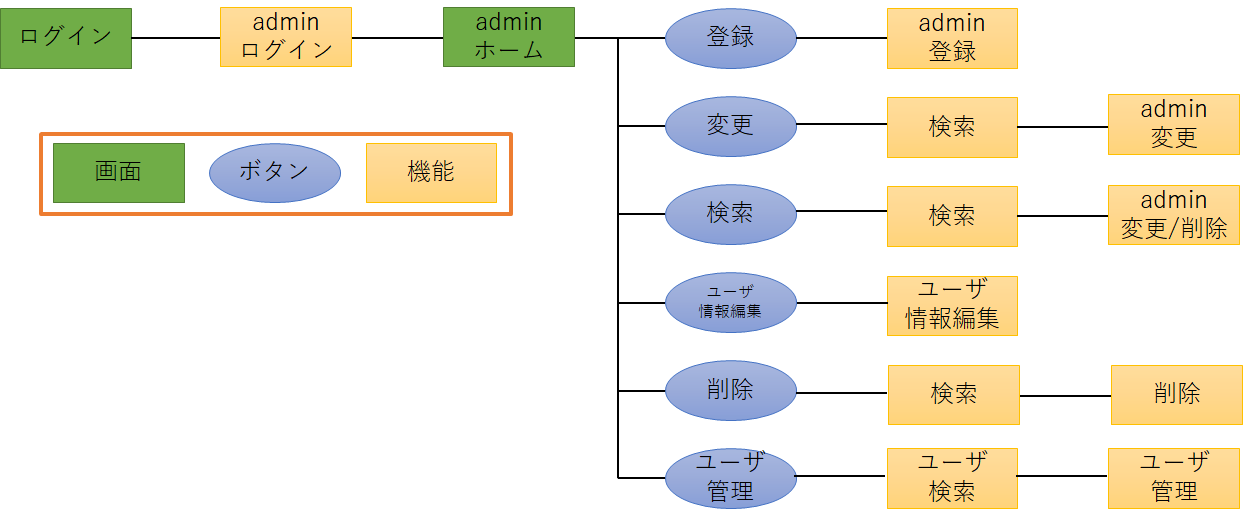
\includegraphics[keepaspectratio, width=0.8\linewidth]{admin_transition-diagram.png}
  \caption{\label{fig:adminの状態遷移図}adminの状態遷移図}
\end{figure}\par

各画面および機能の参照先を次に示す. \\
\begin{minipage}[t]{0.5\linewidth}
  \vspace{1zh}
  \begin{center}
    \begin{tabular}{c|c}
       ログイン & \ref{subsubsec:ユーザ登録・ログイン機能}節 図\ref{fig:ログイン画面のイメージ図} \\
       \hline
       ホーム & \ref{subsubsec:ホーム画面}節 図\ref{fig:ホーム画面のイメージ図} \\
       \hline
       登録 & \ref{subsubsec:登録機能(follower)}節 図\ref{fig:登録画面のイメージ図} \\
       \hline
       検索 & \ref{subsubsec:検索機能(follower)}節 図\ref{fig:検索画面のイメージ図} \\
       \hline
       変更 & \ref{subsubsec:変更機能(follower)}節 図\ref{fig:変更画面のイメージ図} \\
       \hline
       ユーザ情報編集 & \ref{subsubsec:ユーザ情報編集機能(follower)}節 図\ref{fig:ユーザ情報編集画面のイメージ図} \\
    \end{tabular}
  \end{center}
\end{minipage}
%
\hfill
%
\begin{minipage}[t]{0.5\linewidth}
  \vspace{1zh}
  \begin{center}
    \begin{tabular}{c|c}
       adminログイン & \ref{subsubsec:ユーザ登録・ログイン機能}節 図\ref{fig:ログイン画面のイメージ図} \\
       \hline
       ホーム & \ref{subsubsec:ホーム画面}節 図\ref{fig:ホーム画面のイメージ図} \\
    \end{tabular}
  \end{center}
\end{minipage}

%%%%%
\clearpage
\subsubsection{ホーム画面}
\label{subsubsec:ホーム画面}
図\ref{fig:一般ユーザの状態遷移図}, 図\ref{fig:adminの状態遷移図}内にあるホーム画面のイメージ図を次に示す. 図\ref{fig:ホーム画面のイメージ図}を一般ユーザのものとし, 図\ref{fig:adminのホーム画面のイメージ図}を管理者ユーザのものとする.
\begin{figure}[h]
  \centering
  \fbox{
    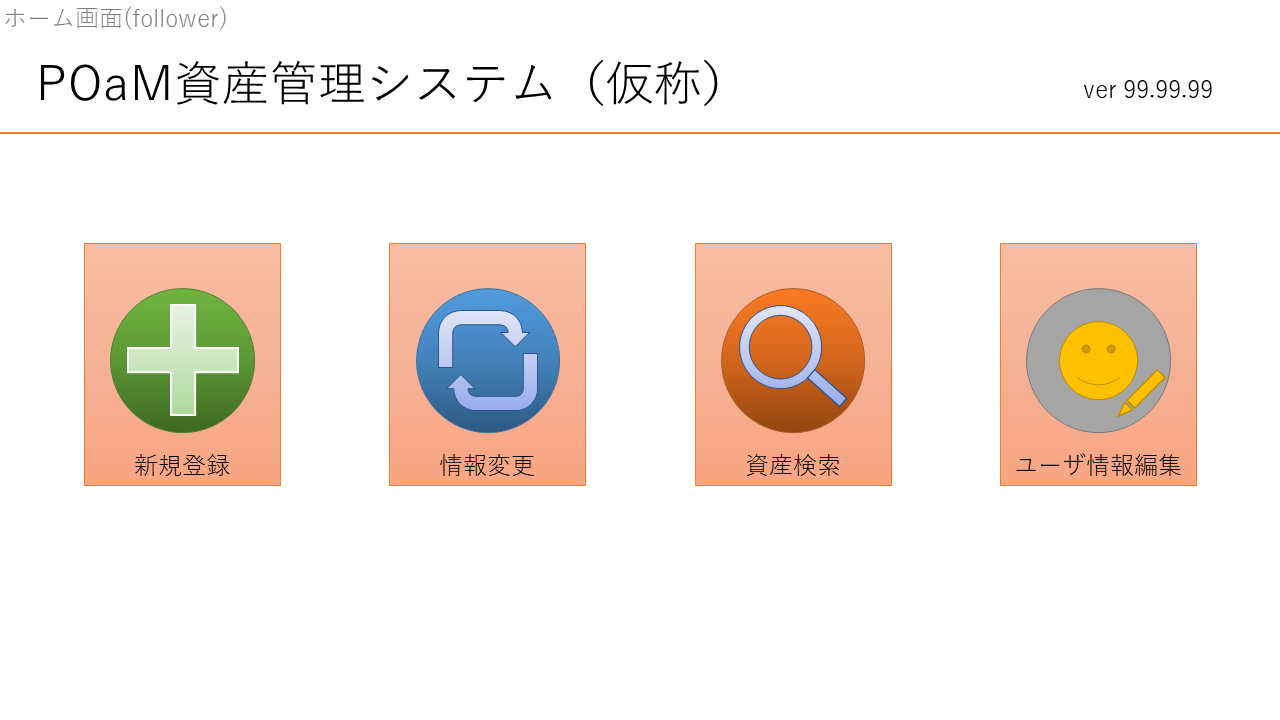
\includegraphics[keepaspectratio, width=0.8\linewidth]{home.png}
  }
  \caption{\label{fig:ホーム画面のイメージ図}ホーム画面のイメージ図}
\end{figure}

\begin{figure}[h]
  \centering
  \fbox{
    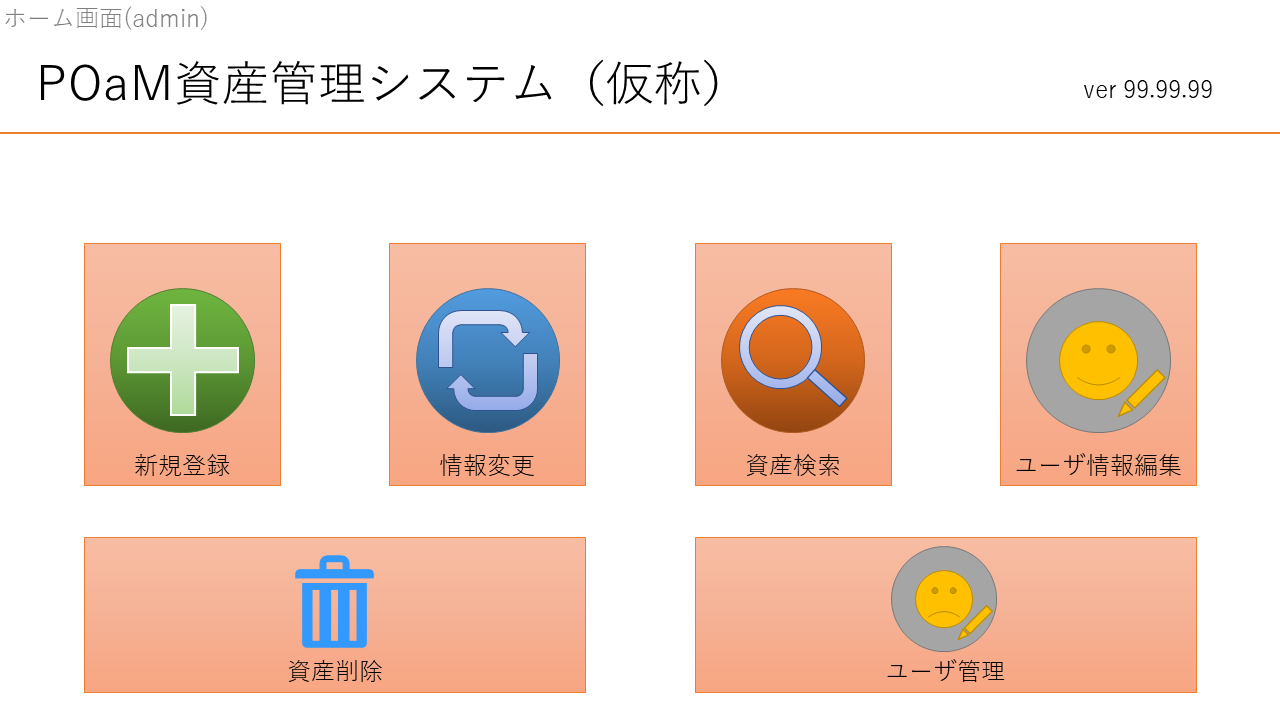
\includegraphics[keepaspectratio, width=0.8\linewidth]{admin_home.PNG}
  }
  \caption{\label{fig:adminのホーム画面のイメージ図}adminのホーム画面のイメージ図}
\end{figure}


%%%%%
\clearpage
\subsubsection{ユーザ登録・ログイン機能}
\label{subsubsec:ユーザ登録・ログイン機能}
メールアドレス$^{*1}$(サレジオドメイン)に基づくIDと任意に設定するパスワードによってユーザ情報を登録する. また, これらによりログインする機能. 登録した情報を使用して個人を識別する. 資産情報を編集したときにログを残すために実装する. ログイン画面のイメージ図を図\ref{fig:ログイン画面のイメージ図}に示す. \par
\begin{figure}[h]
  \centering
  \fbox{
    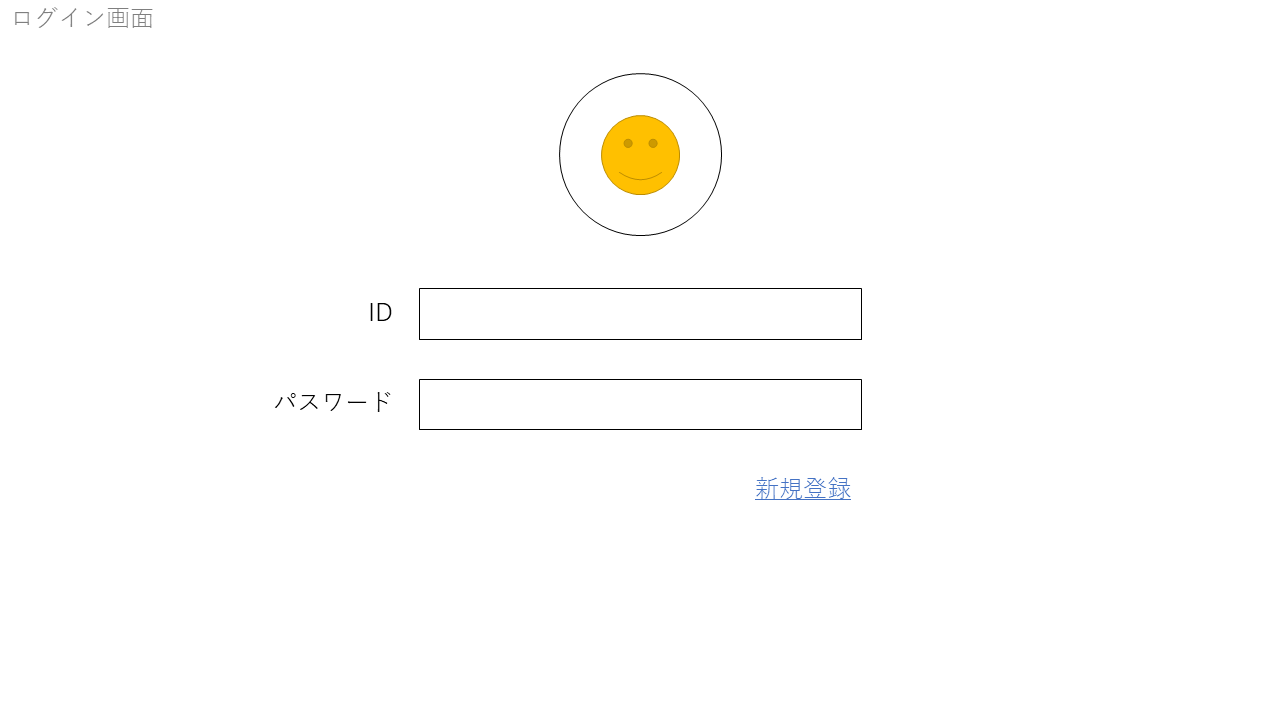
\includegraphics[keepaspectratio, width=0.8\linewidth]{login.png}
  }
  \caption{\label{fig:ログイン画面のイメージ図}ログイン画面のイメージ図}
\end{figure}

%%%%%
\clearpage
\subsection{一般ユーザ(follower)}
\label{subsec:一般ユーザ(follower)}
一般ユーザは資産番号以外のデータを登録ができ, 資産の場所, 担当, 個数を変更することができる. adminの管理下にある. admin以外が一般ユーザを新規登録することはできない.

%%%%%
\subsubsection{登録機能}
\label{subsubsec:登録機能(follower)}
新しい資産を登録する機能. 所属, 場所, 担当, 管理者, 資産名, 形式, 個数, 画像の8項目の入力を要求する. \par
登録画面のイメージ図を図\ref{fig:登録画面のイメージ図}に示す. 各項目について, 要求する入力形式に基づいて登録できるようになっている. \par
ログインしているユーザの情報に基づいて, 所属, 担当はシステムによって先行入力する機能を検討中.
\begin{figure}[h]
  \centering
  \fbox{
    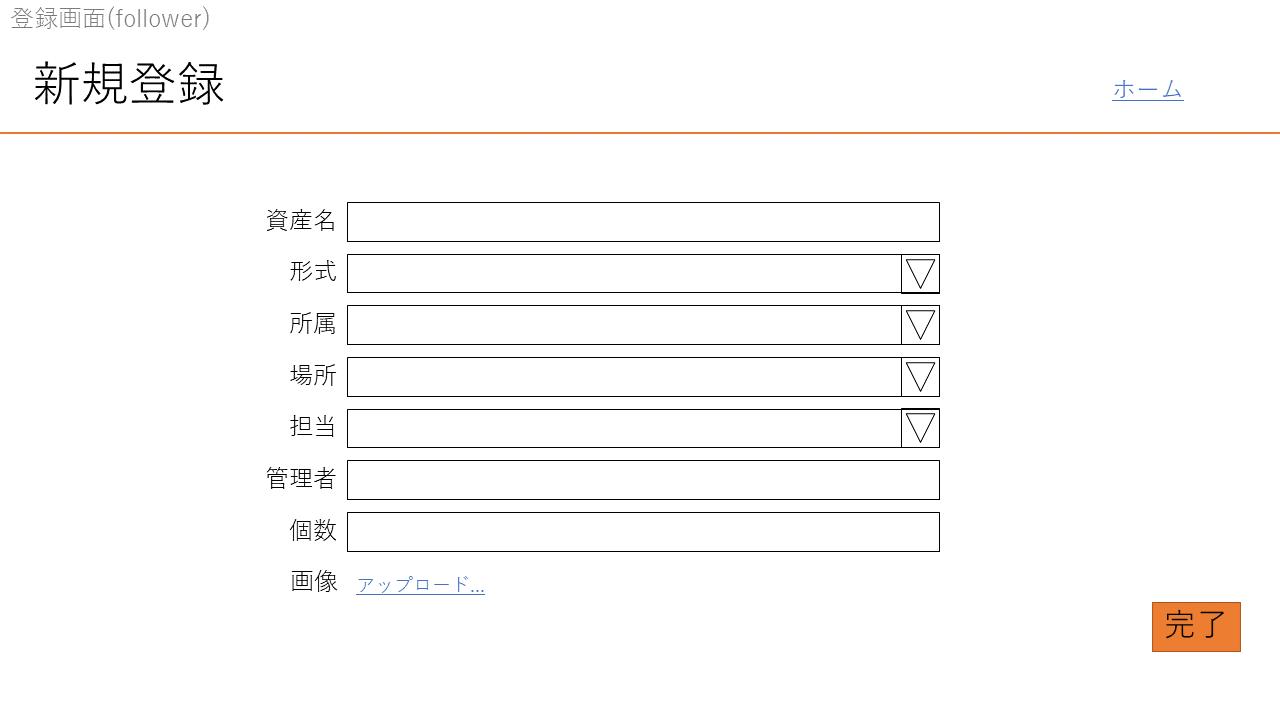
\includegraphics[keepaspectratio, width=0.8\linewidth]{register.png}
  }
  \caption{\label{fig:登録画面のイメージ図}登録画面のイメージ図}
\end{figure}\par

%%%%%
\clearpage
\subsubsection{変更機能}
\label{subsubsec:変更機能(follower)}
資産情報を変更する機能. 図\ref{fig:変更画面のイメージ図}の項目ごとに変更を可能とする. ただし, 管理者権限のない(管理者でない)ユーザには一部の項目は変更できないものとする. 編集ができる部分は黒く表示され, 編集ができない部分については, 図\ref{fig:変更画面のイメージ図}のように灰色で表示される. 各項目について, 要求する入力形式に基づいて変更できるようにする. また, 変更を実行する前に確認をする.
\begin{figure}[h]
  \centering
  \fbox{
    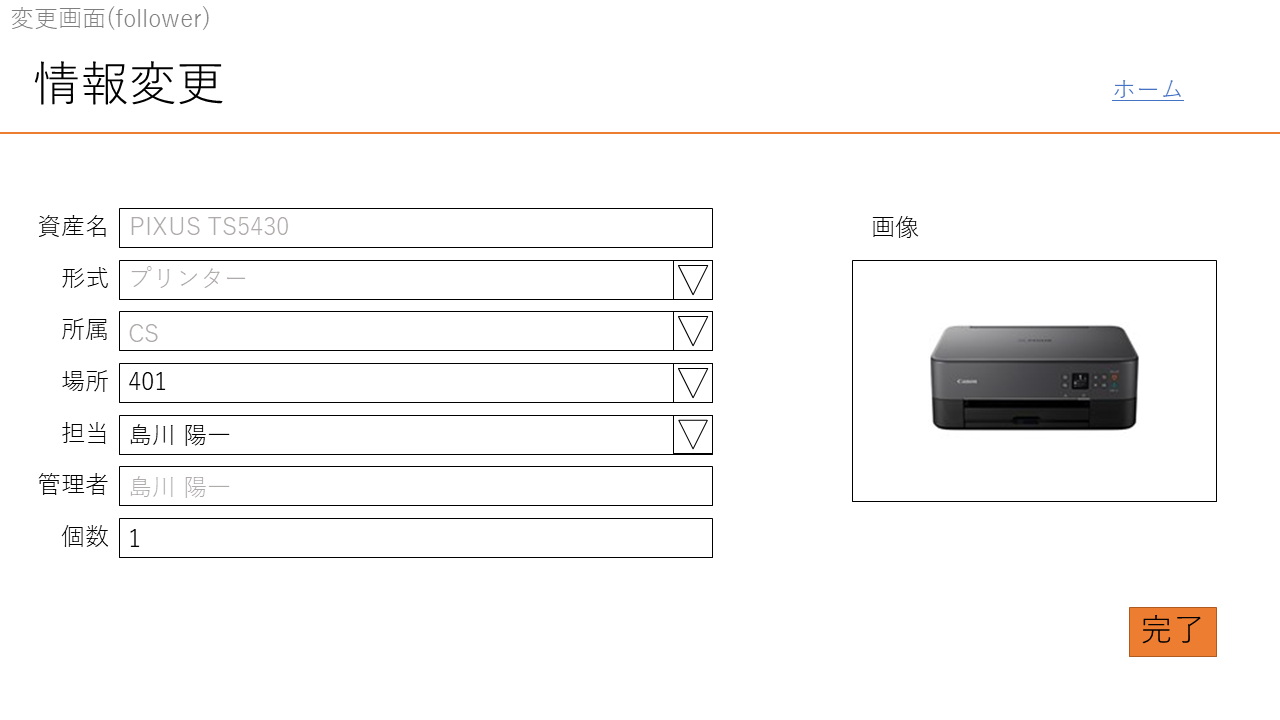
\includegraphics[keepaspectratio, width=0.8\linewidth]{change.png}
  }
  \caption{\label{fig:変更画面のイメージ図}変更画面のイメージ図}
\end{figure}

%%%%%
\clearpage
\subsubsection{検索機能}
\label{subsubsec:検索機能(follower)}
資産番号, 製品名, 管理者, 所有者, 所在別, 購入日でそれぞれ検索またはソートを行う機能. 図\ref{fig:検索画面のイメージ図}に検索画面のイメージ図を示す. 
\begin{figure}[h]
  \centering
  \fbox{
    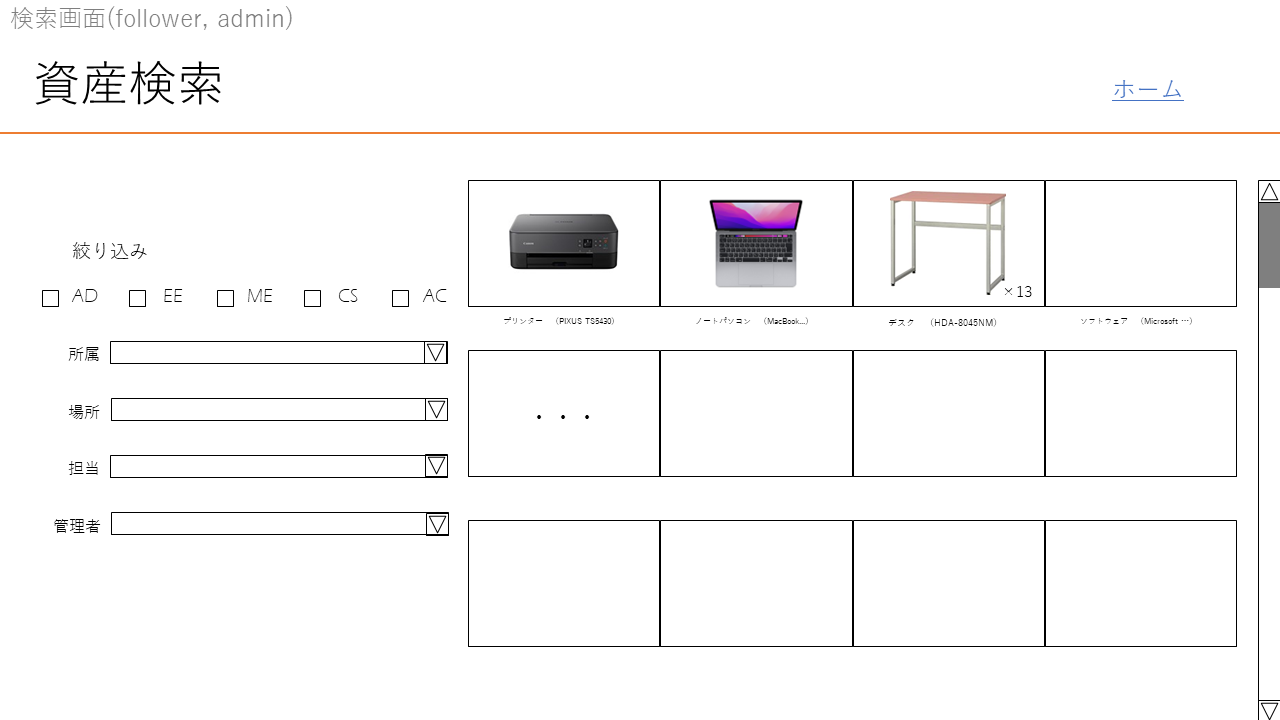
\includegraphics[keepaspectratio, width=0.8\linewidth]{search.png}
  }
  \caption{\label{fig:検索画面のイメージ図}検索画面のイメージ図}
\end{figure}

%%%%%
\clearpage
\subsubsection{ユーザ情報編集機能}
\label{subsubsec:ユーザ情報編集機能(follower)}
ユーザ情報(ID, パスワード, プロフィール画像, 表示名, 所属)を編集する機能. ユーザ情報編集画面のイメージ図を図\ref{fig:ユーザ情報編集画面のイメージ図}に示す. \par
ユーザ情報の構成について検討中.
\begin{figure}[h]
  \centering
  \fbox{
    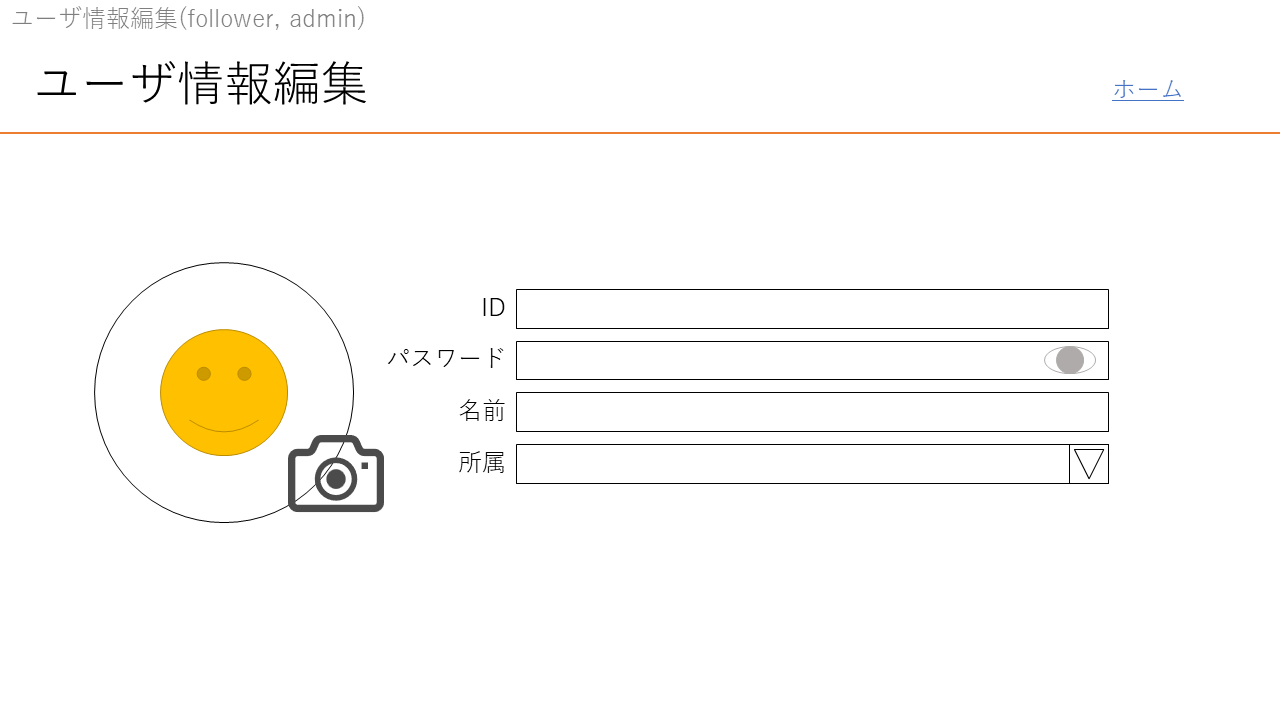
\includegraphics[keepaspectratio, width=0.8\linewidth]{change-user-info.png}
  }
  \caption{\label{fig:ユーザ情報編集画面のイメージ図}ユーザ情報編集画面のイメージ図}
\end{figure}

%%%%%
\clearpage
\subsection{管理者ユーザ(admin)}
\label{subsec:管理者ユーザ(admin)}
管理者ユーザは資産番号の登録と変更, 一般ユーザが変更できない資産情報の変更ができる. \par
管理者ユーザは一部のユーザ(学科長, 事務)を想定している. 

%%%%%
\subsubsection{登録機能}
\label{subsubsec:登録機能(admin)}
一般ユーザでは登録ができなかった資産番号を登録することができる. 現時点では1つ1つ入力を行う必要がある. \par
資産番号の入力方法については検討中. 
\begin{figure}[h]
  \centering
  \fbox{
    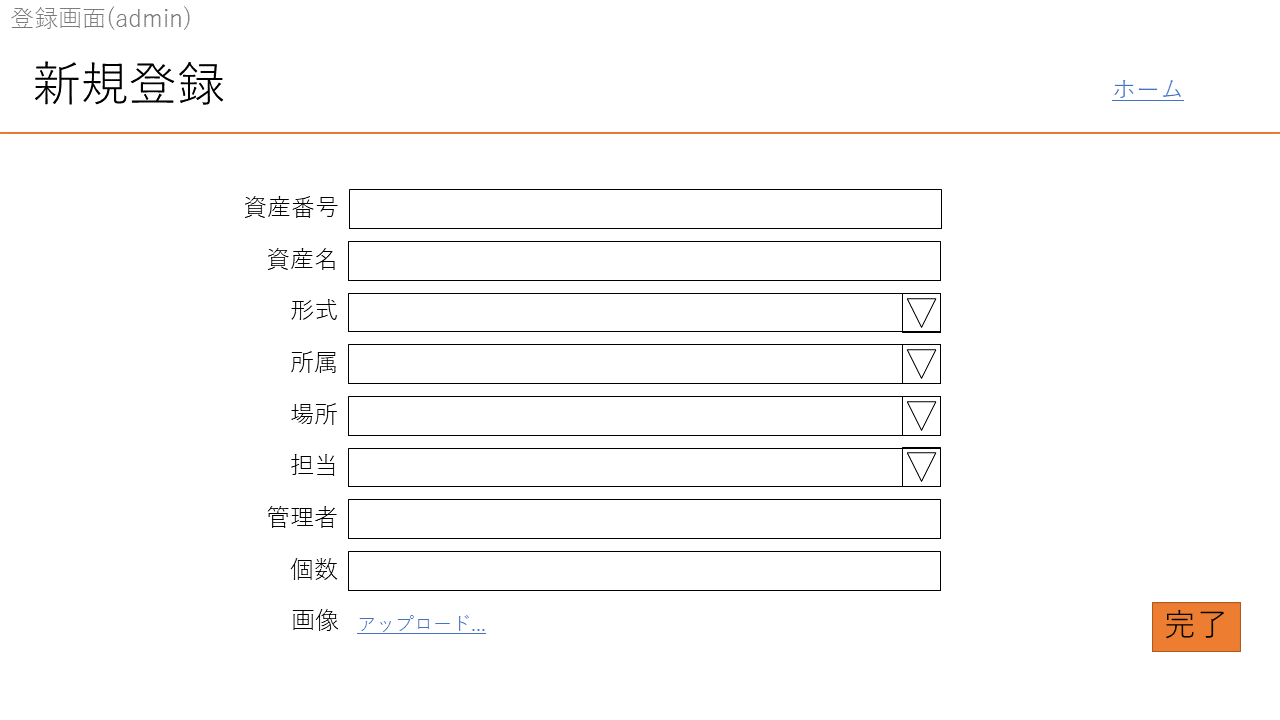
\includegraphics[keepaspectratio, width=0.8\linewidth]{admin_register.png}
  }
  \caption{\label{fig:adminの登録画面のイメージ図}adminの登録画面のイメージ図}
\end{figure}\par

%%%%%
\clearpage
\subsubsection{削除機能}
\label{subsubsec:削除機能}
資産情報を削除する機能. 削除を実行した場合, 該当の資産情報はデータから完全に削除され, サルベージされない. ただし, 削除したログは残す. ログに記載する情報は削除日時, 削除したユーザ, 削除した資産の資産番号の3つを予定している. また, 削除を実行する前にユーザに対して確認をする.
\begin{figure}[h]
  \centering
  \fbox{
    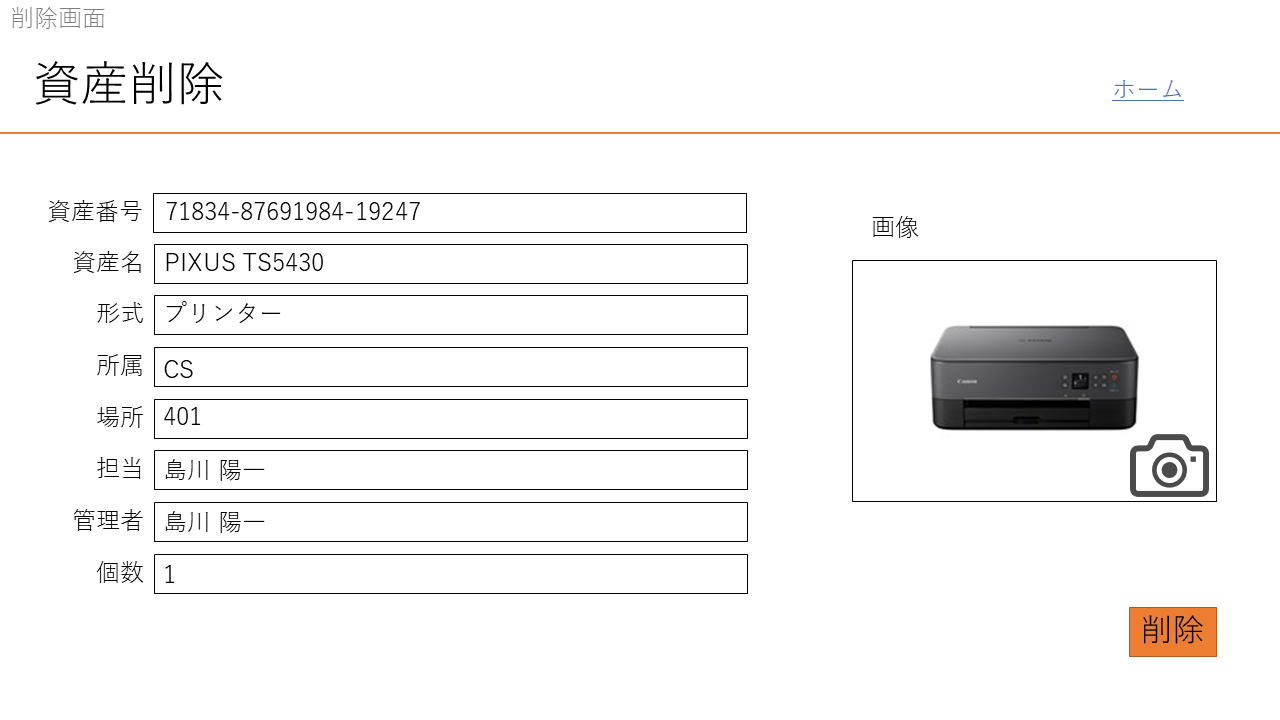
\includegraphics[keepaspectratio, width=0.8\linewidth]{admin_delete.png}
  }
  \caption{\label{fig:削除画面のイメージ図}削除画面のイメージ図}
\end{figure}\par

%%%%%
\clearpage
\subsubsection{変更機能}
\label{subsubsec:変更機能(admin)}
一般ユーザでは変更ができなかった資産番号, 資産名, 形式, 所属, 管理者, 画像の計6項目を変更することができる. \par
各項目について, 要求する入力形式に基づいて変更できるようにする. また, 変更を実行する前に確認をする. 
\begin{figure}[h]
  \centering
  \fbox{
    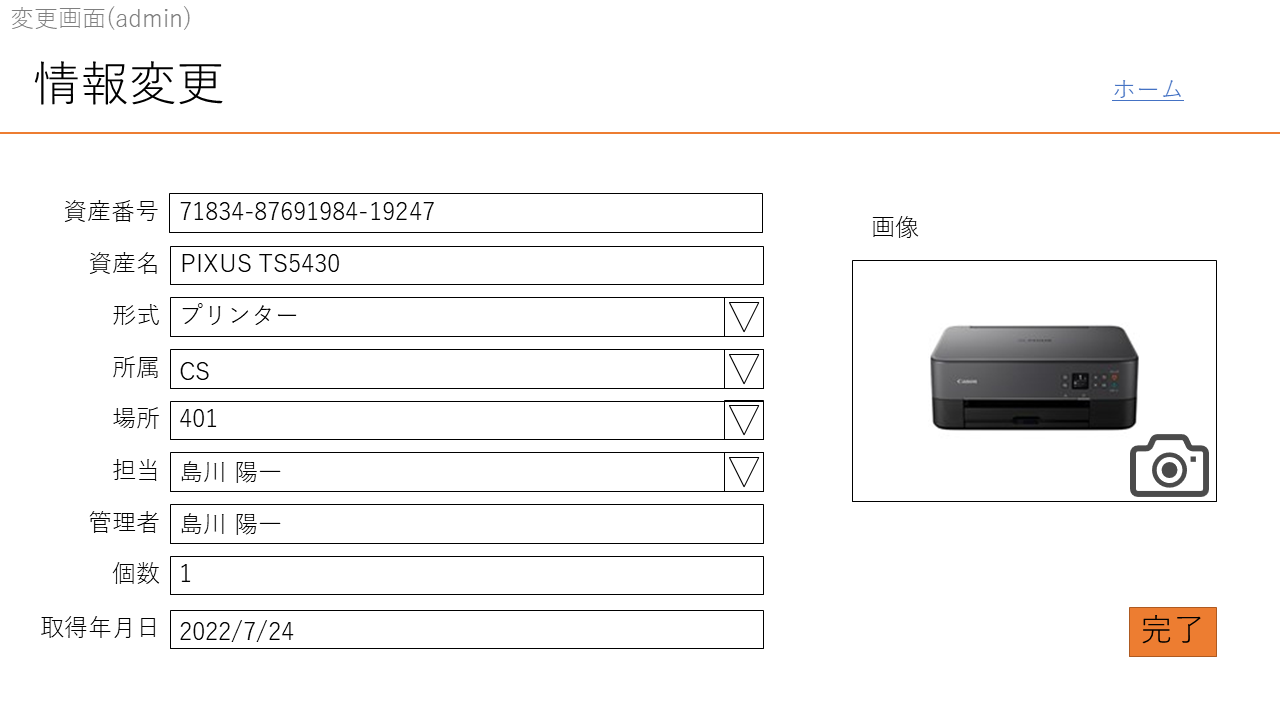
\includegraphics[keepaspectratio, width=0.8\linewidth]{admin_change.png}
  }
  \caption{\label{fig:adminの変更画面のイメージ図}adminの変更画面のイメージ図}
\end{figure}

%%%%%
\clearpage
\subsubsection{検索機能}
\label{subsubsec:検索機能(admin)}
資産番号, 製品名, 管理者, 所有者, 所在別, 購入日でそれぞれ検索またはソートを行う機能. 一般ユーザと画面の構成, 機能は同じである.
\begin{figure}[h]
  \centering
  \fbox{
    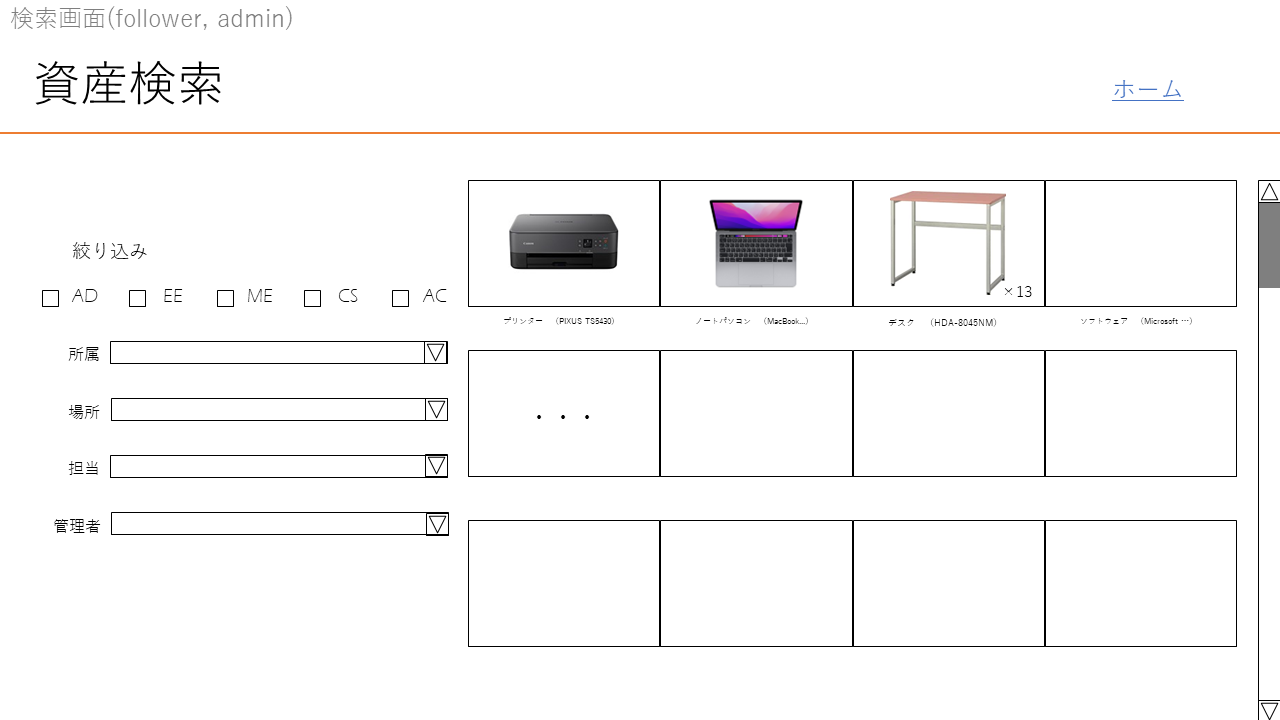
\includegraphics[keepaspectratio, width=0.8\linewidth]{search.png}
  }
  \caption{\label{fig:adminの検索画面のイメージ図}adminの検索画面のイメージ図}
\end{figure}

%%%%%
\clearpage
\subsubsection{ユーザ情報編集機能}
\label{subsubsec:ユーザ情報編集機能(admin)}
ユーザ情報(ID, パスワード, プロフィール画像, 表示名, 所属)を編集する機能. ユーザ情報編集画面のイメージ図を図\ref{fig:adminのユーザ情報編集画面のイメージ図}に示す. \par
一般ユーザと画面の構成, 機能は同じである.
\begin{figure}[h]
  \centering
  \fbox{
    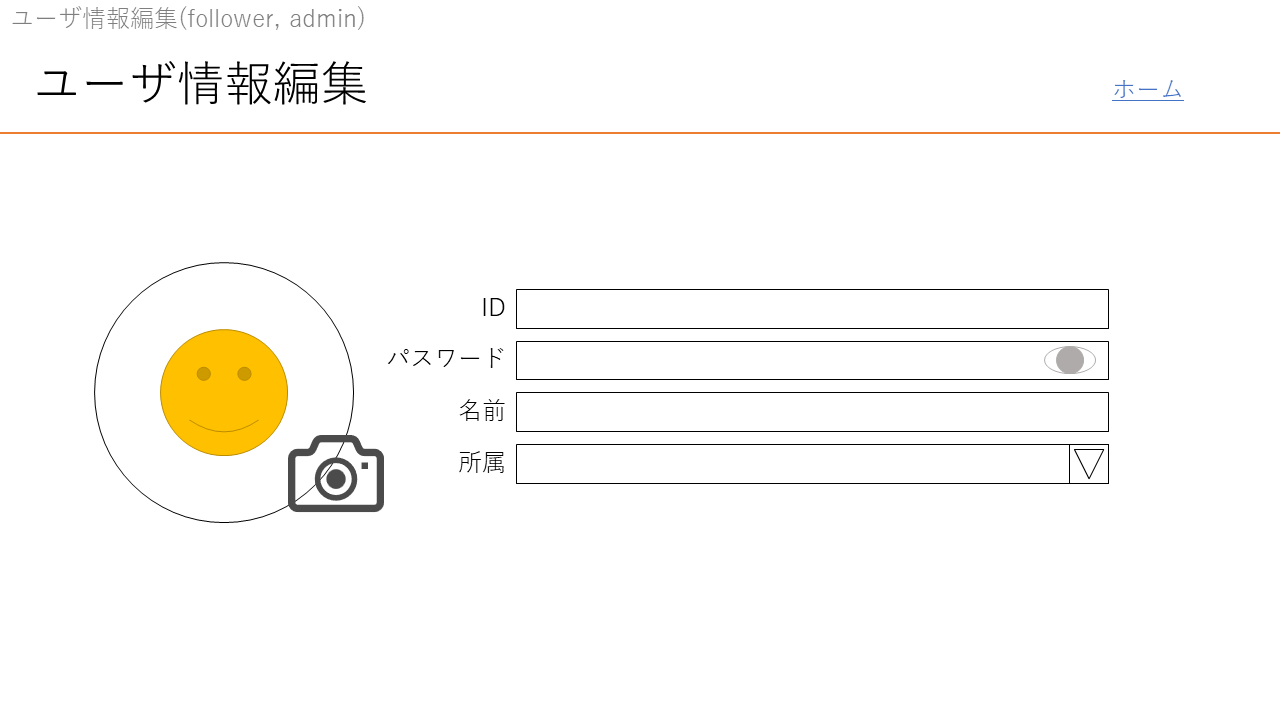
\includegraphics[keepaspectratio, width=0.8\linewidth]{change-user-info.png}
  }
  \caption{\label{fig:adminのユーザ情報編集画面のイメージ図}adminのユーザ情報編集画面のイメージ図}
\end{figure}

%%%%%
\clearpage
\subsubsection{ユーザ一覧検索機能}
\label{subsubsec:ユーザ一覧検索機能}
登録済みの一般ユーザがプロフィールの画像とともに表示され, ユーザの検索ができる. ここから一般ユーザの情報を編集と一般ユーザの新規登録が可能になっている.
\begin{figure}[h]
  \centering
  \fbox{
    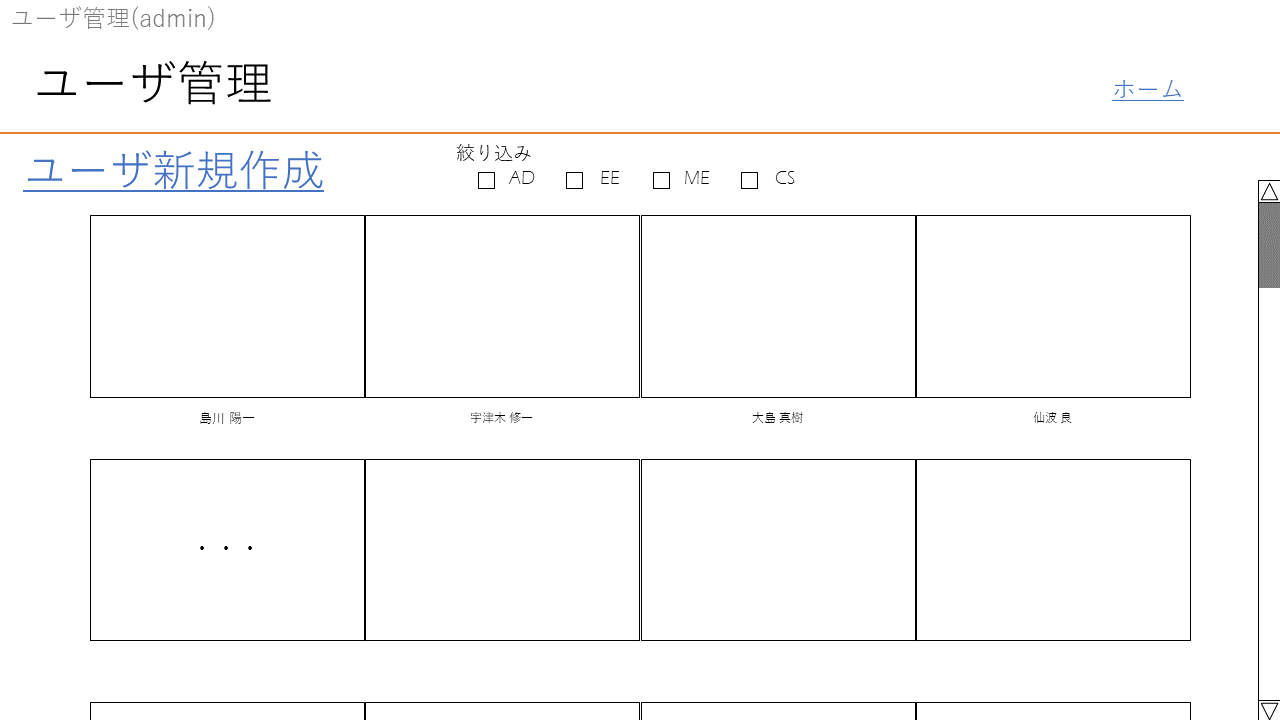
\includegraphics[keepaspectratio, width=0.8\linewidth]{admin_user-search.PNG}
  }
  \caption{\label{fig:adminのユーザ一覧検索機能のイメージ図}adminのユーザ一覧検索機能のイメージ図}
\end{figure}

%%%%%
\clearpage
\subsubsection{一般ユーザ情報編集機能}
\label{subsubsec:一般ユーザ情報編集機能}
一般ユーザ情報の変更と削除が行える. 変更ができるものは現時点ではID(サレジオドメイン), 名前, 所属となっている. 削除は右下にある削除ボタンを選択すると行える. また, 削除を実行する前に確認をする. 
\begin{figure}[h]
  \centering
  \fbox{
    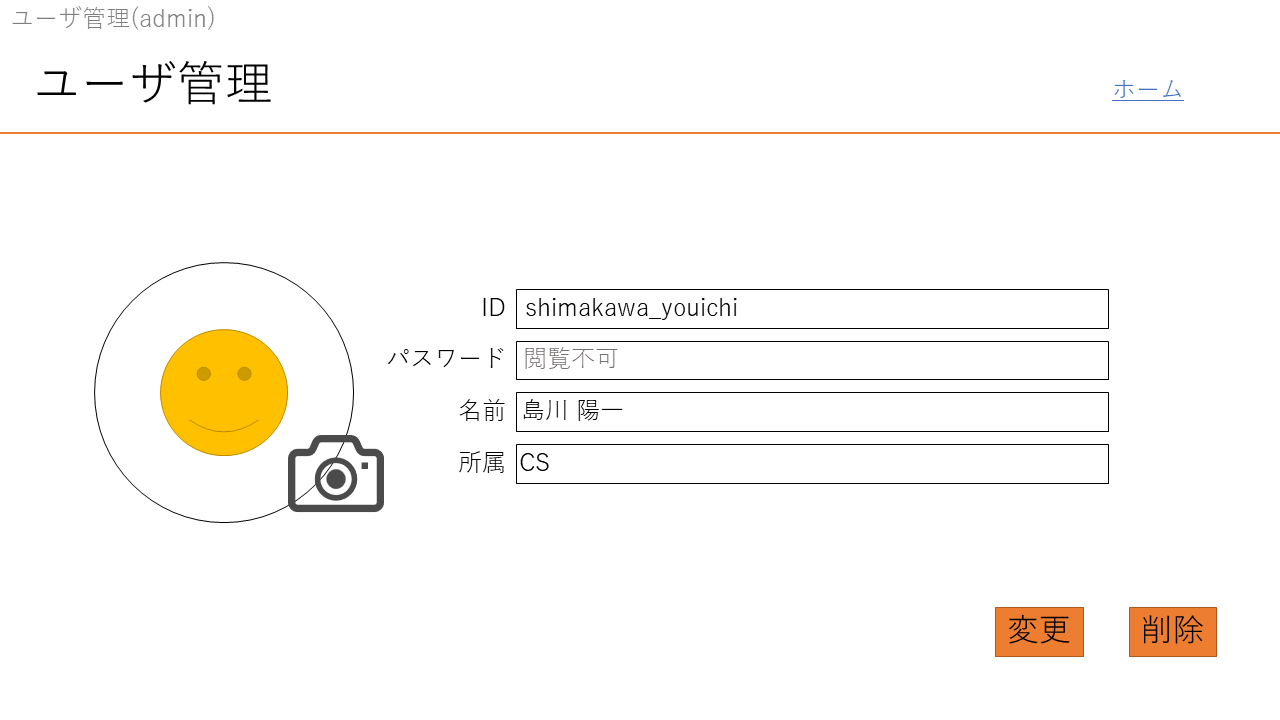
\includegraphics[keepaspectratio, width=0.8\linewidth]{admin_user-change.PNG}
  }
  \caption{\label{fig:adminの一般ユーザ情報編集機能のイメージ図}adminの一般ユーザ情報編集機能のイメージ図}
\end{figure}

%%%%%
\clearpage
\subsubsection{一般ユーザ新規作成機能}
\label{subsubsec:一般ユーザ新規作成機能}
一般ユーザの新規登録が行える. 登録に必要なものはID(サレジオドメイン), 名前, 所属となっている. 管理者ユーザしか登録できない理由は無断で新規登録をされ, 混乱を招かないためである.
\begin{figure}[h]
  \centering
  \fbox{
    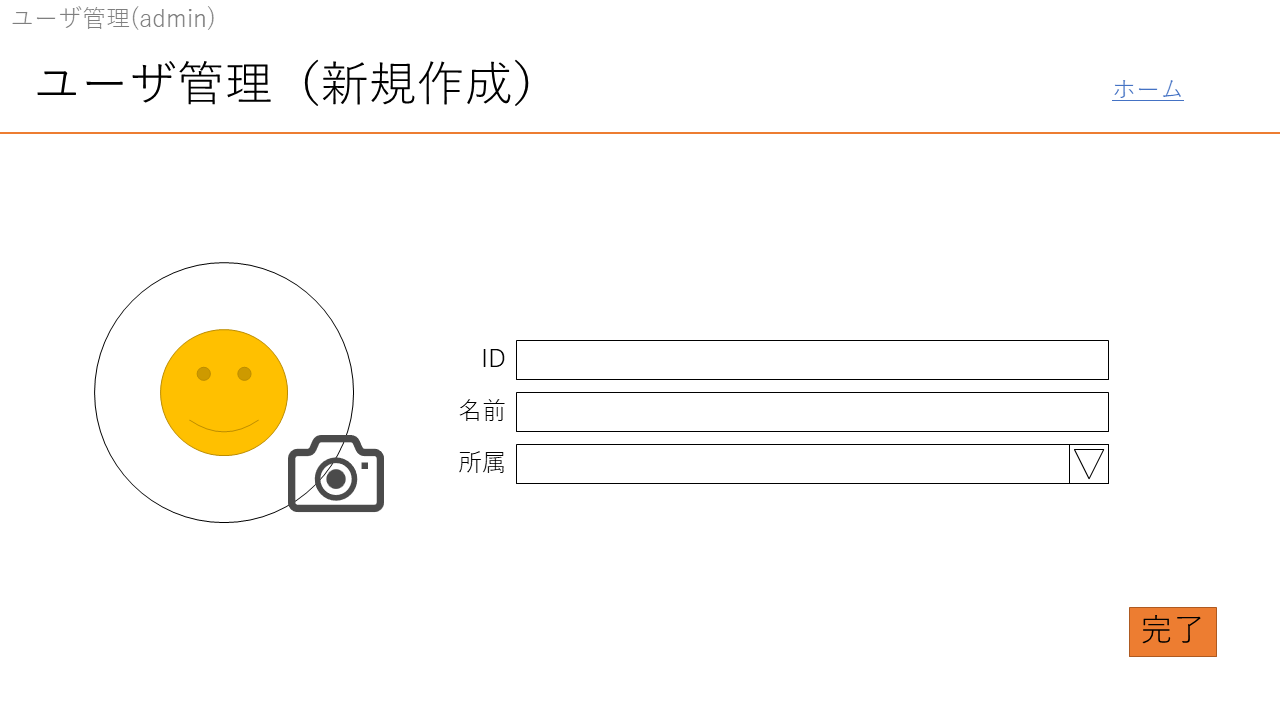
\includegraphics[keepaspectratio, width=0.8\linewidth]{admin_user-register.PNG}
  }
  \caption{\label{fig:adminの一般ユーザ新規作成機能のイメージ図}adminの一般ユーザ新規作成機能のイメージ図}
\end{figure}

%%%%%%%%%%
%\newpage
%\section{用語集}
%\label{sec:用語集}
%\begin{enumerate}
%\item[メールアドレス] @以左のユーザ名(メールアカウント)と, @以右のドメインによって構成される.  例 {\tt test@example.com}
%\end{enumerate}

%%%%%
\clearpage
{\Large\bfseries \ 改変履歴}
\begin{table}[htbp]
  %\caption{}
  %\label{tb:}
  \centering
  \begin{tabularx}{\textwidth}{wc{0.2\linewidth}|wl{0.6\linewidth}|wl{0.2\linewidth}}
    日付       & 項目                                           & 担当者     \\
    \hline \hline
    2022/05/27 & 初版作成                                       & 田桑       \\
    \hline
    2022/06/09 & 全体の表現の変更・追加                         & 高橋・田中 \\
    \hline
    2022/07/05 & \ref{sec:各機能の詳細・システムの詳細}節の編集 & 高橋・田中 \\
    \hline
    2022/07/21 & \ref{sec:各機能の詳細・システムの詳細}節の編集 & 高橋・田中 \\
    \hline
    2022/12/01 & \ref{sec:各機能の詳細・システムの詳細}節の編集 & 高橋・田中 \\
    % \hline
  \end{tabularx}
\end{table}

\end{document}
%%%%%%%%%%%%%%%%%%%
%%%%%%%%%%%%%%%%%%%

%
